%-*-latex-*-
\tinysidebar{\debug{exercises/discrete-probability/{bernoulli-05/answer.tex}}}

The probability of getting at least 2 sixes is
\[
B(n,p; 2) + 
B(n,p; 3) + 
B(n,p; 4) + 
\cdots + 
B(n,p; 7) 
\]
Therefore the student will earn
\[
\left(
  B(n,p; 2) + 
  B(n,p; 3) + 
  B(n,p; 4) + 
  \cdots + 
  B(n,p; 7)
  \right) \times 100 - 1
\]
(The \lq\lq $-1$'' is because the student has to pay \$1 to play.) 
Of course to make money, you will want
\[
\left(
  B(n,p; 2) + 
  B(n,p; 3) + 
  B(n,p; 4) + 
  \cdots + 
  B(n,p; 7)
  \right) \times 100 - 1 < 0
\]
i.e.,
\[
  B(n,p; 2) + 
  B(n,p; 3) + 
  B(n,p; 4) + 
  \cdots + 
  B(n,p; 7)  < 1/100
\]
It's easier to use this:
\[
  1
  - B(n,p; 0) 
  - B(n,p; 1) 
  - B(n,p; 2) 
  < 1/100
\]
and therefore we want
\[
  99/100 < B(n,p; 0) + B(n,p; 1) + B(n,p; 2)
\]
which is the same as
\[
99/100
<
\binom{7}{0}p^0(1-p)^{7-0}
+
\binom{7}{1}p^1(1-p)^{7-1}
+
\binom{7}{2}p^2(1-p)^{7-2}
\]

The following is a graph for different values of $p$:
\begin{center}
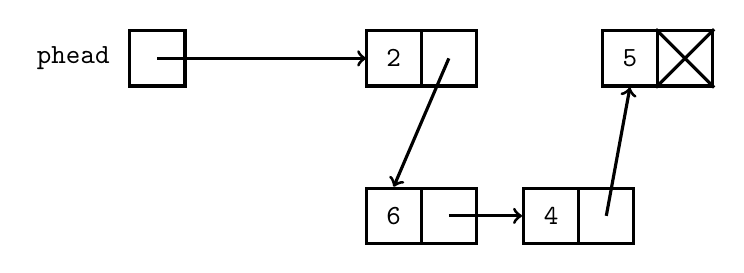
\begin{tikzpicture}

\draw (0.35, 0.35)
  node[draw, line width=0.04cm, , color=black,
       rounded corners=0cm, inner sep=0cm] {

\begin{minipage}[t][0.7cm]{0.7cm}
\mbox{}

\end{minipage}

};\draw (0.35, 0.35) node[color=black] {{\texttt{2}}};
\draw (1.0499999999999998, 0.35)
  node[draw, line width=0.04cm, , color=black,
       rounded corners=0cm, inner sep=0cm] {

\begin{minipage}[t][0.7cm]{0.7cm}
\mbox{}

\end{minipage}

};\draw (1.0499999999999998, 0.35) node[color=black] {{\texttt{}}};
\draw (0.35, -1.65)
  node[draw, line width=0.04cm, , color=black,
       rounded corners=0cm, inner sep=0cm] {

\begin{minipage}[t][0.7cm]{0.7cm}
\mbox{}

\end{minipage}

};\draw (0.35, -1.65) node[color=black] {{\texttt{6}}};
\draw (1.0499999999999998, -1.65)
  node[draw, line width=0.04cm, , color=black,
       rounded corners=0cm, inner sep=0cm] {

\begin{minipage}[t][0.7cm]{0.7cm}
\mbox{}

\end{minipage}

};\draw (1.0499999999999998, -1.65) node[color=black] {{\texttt{}}};
\draw (2.35, -1.65)
  node[draw, line width=0.04cm, , color=black,
       rounded corners=0cm, inner sep=0cm] {

\begin{minipage}[t][0.7cm]{0.7cm}
\mbox{}

\end{minipage}

};\draw (2.35, -1.65) node[color=black] {{\texttt{4}}};
\draw (3.0500000000000003, -1.65)
  node[draw, line width=0.04cm, , color=black,
       rounded corners=0cm, inner sep=0cm] {

\begin{minipage}[t][0.7cm]{0.7cm}
\mbox{}

\end{minipage}

};\draw (3.0500000000000003, -1.65) node[color=black] {{\texttt{}}};
\draw (3.35, 0.35)
  node[draw, line width=0.04cm, , color=black,
       rounded corners=0cm, inner sep=0cm] {

\begin{minipage}[t][0.7cm]{0.7cm}
\mbox{}

\end{minipage}

};\draw (3.35, 0.35) node[color=black] {{\texttt{5}}};
\draw (4.05, 0.35)
  node[draw, line width=0.04cm, , color=black,
       rounded corners=0cm, inner sep=0cm] {

\begin{minipage}[t][0.7cm]{0.7cm}
\mbox{}

\end{minipage}

};\draw (4.05, 0.35) node[color=black] {{\texttt{}}};\draw[line width=0.04cm,black,->] (1.05,0.35) to  (0.35,-1.28);
\draw[line width=0.04cm,black,->] (1.05,-1.65) to  (1.98,-1.65);
\draw[line width=0.04cm,black,->] (3.05,-1.65) to  (3.35,-0.02);
\draw[line width=0.04cm,black] (3.68,0.72) to  (4.42,-0.02);
\draw[line width=0.04cm,black] (4.42,0.72) to  (3.68,-0.02);

\draw (-2.65, 0.35)
  node[draw, line width=0.04cm, , color=black,
       rounded corners=0cm, inner sep=0cm] {

\begin{minipage}[t][0.7cm]{0.7cm}
\mbox{}

\end{minipage}

};\draw (-2.65, 0.35) node[color=black] {{\texttt{}}};\draw[line width=0.04cm,black,->] (-2.65,0.35) to  (0,0.35);

\draw (-3.7199999999999998, 0.35)
  node[draw, line width=0.04cm, , color=white,
       rounded corners=0cm, inner sep=0cm] {

\begin{minipage}[t][0.1cm]{0.1cm}
\mbox{}

\end{minipage}

};\draw (-3.7199999999999998, 0.35) node[color=black] {{\texttt{phead}}};
\end{tikzpicture}

\end{center}


Zooming in on the part of the graph where $x$ is in $[0.05, 0.1]$, we get
%\begin{python}
%from math import *
%from latextool_basic import *
%plot = FunctionPlot(width="7in")
%
%import scipy.misc
%comb = scipy.misc.comb
%
%def B(n, p, k):
%    return comb(n, k) * p**k * (1-p)**(n - k)
%
%def f(p):
%    return B(7, p, 0) + B(7, p, 1) + B(7, p, 2)
%
%myrange = [0.05, 0.06, 0.08, 0.1]
%data1 = [(i,f(i)) for i in myrange]
%data2 = [(i,0.99) for i in myrange]
%
%plot.add(data1, line_width='1', color='black')
%plot.add(data2, line_width='1', color='black')
%print(plot)
%\end{python}

\begin{center}
\begin{tikzpicture}[line width=1]
\begin{axis}[width=5in, height=3in,
             xlabel={\mbox{}},
             xlabel style={name=xlabel}, 
             ylabel={\mbox{}},
             xtick=data,
             yticklabels={,,},
             tick label style={/pgf/number format/fixed},
             legend style={
                at={(xlabel.south)},
                yshift=-1ex,
                anchor=north,
                legend cell align=left,
                },
        ]
]
\addplot[draw=black, line width=1] coordinates
 {(0.05, 0.996)
  (0.06, 0.994)
  (0.08, 0.986)
  (0.10, 0.974)};
\addplot[draw=black, line width=1] coordinates
 {(0.05, 0.990)
  (0.06, 0.990)
  (0.08, 0.990)
  (0.10, 0.990)};
\end{axis}
\end{tikzpicture}\end{center}

Therefore the break even value for $p$ is approximately $0.07$.
(For a fair die, the probability for getting a six is $1/6 = 0.167$.)

We now compute our gains for a few values of $p$ near $0.07$.
If $p = 0.06$, then the player would make
\[
(1 - B(7,0.06;0) - B(7,0.06;1) - B(7,0.06;2)) \times 100 - 1
=
-0.3706...
\]
which means that we gain \$0.37 per game.
If $p = 0.07$, then the player would make
\[
(1 - B(7,0.07;0) - B(7,0.07;1) - B(7,0.07;2)) \times 100 - 1
=
-0.0312...
\]
which means that we gain \$0.03 per game.
If $p = 0.08$, then the player would make
\[
(1 - B(7,0.08;0) - B(7,0.08;1) - B(7,0.08;2)) \times 100 - 1
= 0.4014....
\]
which means that we would lose \$0.40 per game.

So, for instance, if we use $p = 0.07$ and a total of 100 games were
played, we will collect \$37.00.




[TO TIDY UP]
